\documentclass[12pt,a4paper]{report}
\usepackage[a4paper,top=2.5cm,bottom=2.5cm,left=2.5cm,right=2.5cm]{geometry}
\usepackage[utf8]{inputenc}
\usepackage{amsmath}
\usepackage{amsfonts}
\usepackage{amssymb}
\usepackage{graphicx}
\usepackage{titlesec}
\usepackage{eurosym}
\usepackage{booktabs}
\usepackage{setspace}
\usepackage{wrapfig}
\usepackage{fancyhdr}
\usepackage{caption}
\usepackage{lipsum}


\begin{document}
	
	\tableofcontents
	\cleardoublepage
	\pagenumbering{arabic}
	
	\chapter{Motivation and background}


\section{Life-cycle of data}

\begin{figure}[h]
	\centering
	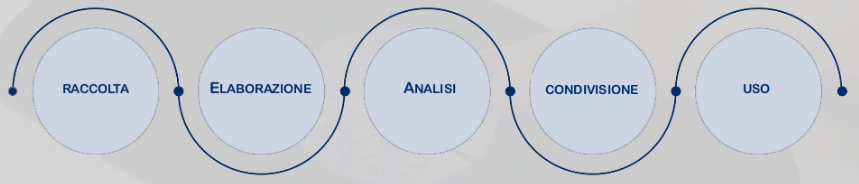
\includegraphics[width=1\linewidth]{imgs datavis/Life cycle.png}
	\caption{Life cycle of data}
	\label{fig:cycle}
\end{figure}

\begin{itemize}
	\item Raccolta dati: questa fase produce una versione elaborabile dei dati. Include la definizione di standard protocolli, modelli (schemi concettuali/logici) con cui misurare ed osservare la realtà, trasformarla in codici/ categorie/numeri.
	\item 	Elaborazione: propedeutica all'analisi
	\item Analisi: l'analisi porta a dei risultati che possono essere positivi, negativi, attesi o inattesi. \`E una fase sempre più automatizzata e supportata dalle macchine (strumento di sintesi)
	\item Condivisione: rende fruibili i dati ad un pubblico più ampio rispetto a chi si è dedicato all'elaborazione. Si può inoltre associare alla pubblicazione in un formato (più o meno) accessibile dal punto di vista del web (internet)
	\item 	Uso: tutto ciò permetterebbe di fruire di queste informazioni per prendere decisioni più informate.
\end{itemize}


In questo ciclo di vita dei dati (si parla di ciclo perché l'utilizzo dei dati comporta la produzione di dati nuovi) la visualizzazione occupa almeno 3 fasi (potrebbe essere utilizzata in tutte): analisi perché è uno strumento di sintesi e consente ad una persona di interpretare i dati più velocemente rispetto ad una rappresentazione tabellare. Nella condivisione la visualizzazione è il concreto sviluppo dei modi migliori per reindirizzare in maniera visuale i risultati di un'elaborazione quindi c'è la scelta dei canali, codici linguaggi più opportuni per dimostrare una certa tesi (risultati di un'elaborazione). Anche nell'uso c'è la visualizzazione cioè è protagonista la competenza che un utilizzatore finale non specialista deve mettere in campo per comprendere quello che gli è stato fatto vedere.

Visualizzazione può essere inconsueta, originale e ciò ampia il terreno di competenze 

Il fatto di utilizzare una visualizzazione più inconsueta, se è efficace ed efficiente (ciò dovrà essere verificato) non conta che sia nota o tradizionale, consente di ampliare il terreno delle competenze della persona che deve fruire di quella visualizzazione. Ovviamente il fruitore dovrà mettere in campo la voglia di imparare qualcosa. Se però la visualizzazione attrae, è esteticamente bella, il fruitore sarà più incentivato ad imparare quello che vogliamo dirgli con quei grafici. 

Noi ci focalizzeremo sulle fasi: analisi e condivisione. 

\section{Why visualizing data is so important in data science and communication}

Importanza di dedicare la giusta attenzione alla visualizzazione dei dati e con attenzione si intende la voglia e la volontà di sviluppare delle competenze, una sensibilità e una responsabilità nei confronti dei soggetti a cui ci rivolgiamo quando mostriamo i risultati di un'analisi dei dati e sensibilità nel capire quali sono i modi migliori che dobbiamo utilizzare nel rivolgerci al pubblico. 

Importanza delle competenze che derivano dal sapere nozionistico (know-what) e dall'applicazione di queste nozioni, sviluppo del progetto.

\begin{center}
	\textsl{Well, you cannot speak of science unless you prove your points. And you cannot prove your points if you don't convince people}
\end{center}

Non si può parlare di scienza a meno che non si sia in grado di provare le proprie tesi. Non si possono provare le proprie tesi se non si è in grado di convincere e influenzare il comportamento delle persone, trasferire un messaggio, concretizzare una comunicazione. 


\subsection{Is it raining more or less than it is used for?}

Qualche tempo fa è emersa l'idea che piovesse di più adesso rispetto al passato e che questo avesse portato ad un cambiamento climatico ossia al fatto che le estati fossero più asciutte e gli autunni più piovosi. 

Un articolo ha presentato i seguenti grafici. La prima visualizzazione riguarda l'inverno mentre la visualizzazione a destra riguarda l'estate. Sulle ascisse viene rappresentata l'altitudine mentre sulle ordinate viene rappresentato un cambiamento nella percentuale di precipitazioni. Un cambiamento nullo significa che non ci sono stati cambiamenti nel periodo compreso fra il 1961 e il 1990. 

Cerchio rosso: stima puntuale. Se l'intervallo di confidenza comprende lo 0 non si può prevedere in maniera significativa che la differenza sia nulla. Da questo si può dire che effettivamente piove di meno nelle zone a livello del mare, ma piove di più in alta quota. D'estate invece anche se c'è qualche deviazione nel tempo (anche se sembra che piova sempre meno) non c'è mai una significatività statistica, pertanto non si può ritenere che a livello del mare o in quota piova effettivamente meno. 

\begin{figure} [h]
	\centering
	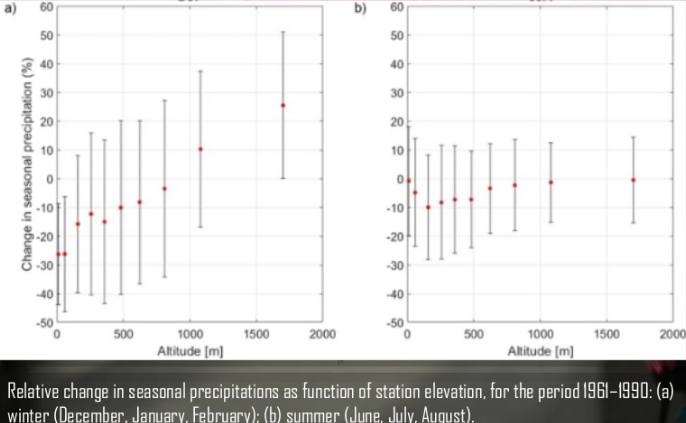
\includegraphics[width=0.4\linewidth]{imgs datavis/Rain.png}
	\caption{}
	\label{fig:rain}
\end{figure} 

Il fatto che non ci siano cambiamenti significativi potrebbe essere dovuto ad una diversa la concentrazione, per esempio negli anni 60 pioveva 500 ml di pioggia in estate e primavera a Milano, magari pioveva meno giornalmente ma più giorni consecutivamente, la stessa cosa può accadere adesso ma in 5 giorni di pioggia. 

\subsection{Is it true that during the weekend it rains more than in the rest of the week?}

\begin{figure} [h]
	\centering
	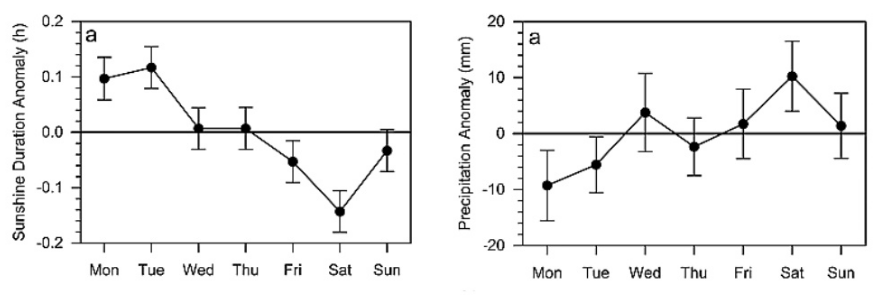
\includegraphics[width=0.5\linewidth]{imgs datavis/Rain during week.png}
	\caption{}
	\label{fig:rain during week}
\end{figure} 

Se consideriamo le figure sopra stime medie della differenza nell'esposizione solare e nella quantità di precipitazioni è possibile vedere che nel sabato c'è meno sole rispetto a quanto ce ne sia durante la settimana, lunedì, martedì c'è sole mentre a partire da giovedì si incomincia a vedere un peggioramento. La precipitazione piovosa è significativamente maggiore il sabato rispetto ad altri giorni e addirittura il lunedì è il giorno in cui piove meno e c'è più sole. 

Gli autori di questo lavoro ritenevano che fossero le città, quindi l'attività a creare le condizioni dell'aumento della nuvolosità nel week-end (quando l'attività antropica è minore).

Ciò che tuttavia emerge al di là dei nessi causali che possiamo individuare è che c'è una significatività statistica nelle anomalie tanto nell'illuminazione solare quanto nella precipitazione e questo andamento è notevole identificarlo durante la settimana. 

\subsection{Everyone's mood improves when the weather is good, right?}

Hanno fatto un'analisi di miliardi di tweet e hanno fatto una sentimental analysis. Si tratta di contare quante parole presenti in un dizionario denotato come positivo si trovano nei tweet rispetto invece a quante parole contenute in un dizionario definito negativo o neutro si trovano nei tweet. 
\begin{figure}[h]
	\centering
	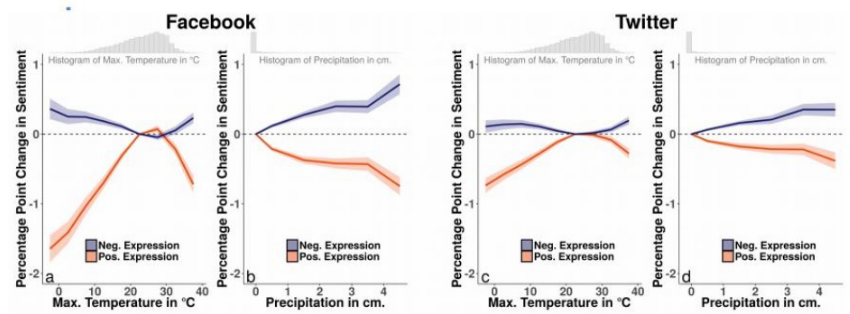
\includegraphics[width=0.5\linewidth]{imgs datavis/Facebook vs Twitter.png}
	\caption{}
	\label{fig:FvsT}
\end{figure} 

Da questa analisi si può vedere  sia su Facebook che su Twitter che all'aumentare della temperatura o delle precipitazioni il sentiment ha delle andature caratteristiche, per esempio all'aumentare della temperatura aumenta e viceversa diminuisce al diminuire della temperatura. Inoltre se la temperatura è aumentata, un ulteriore aumento comporta una situazione di disagio quindi le espressioni positive diminuiscono e quelle negative aumentano. Questa visualizzazione ci mostra delle tendenze incontrovertibili. La visualizzazione ci permette di indirizzare le nostre curiosità. 

\subsection{Who is the best football player of all times? }

Per poter avere un'idea di chi sia il giocatore più grande, possono essere utilizzate le visualizzazioni. 

\begin{figure}[h]
	\centering
	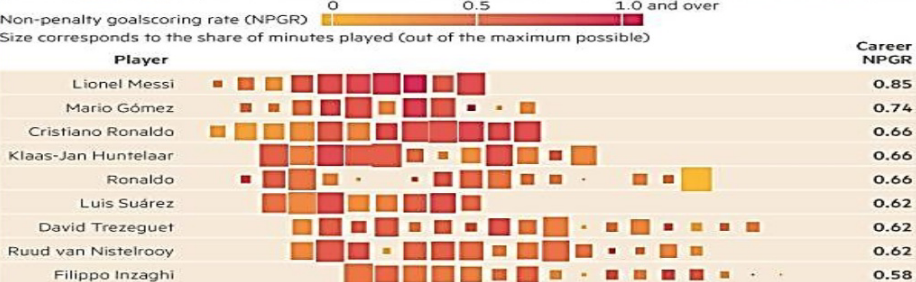
\includegraphics[width=0.5\linewidth]{imgs datavis/Football.png}
	\caption{}
	\label{fig:Football}
\end{figure} 

In questo caso vi sono diverse dimensioni: il rapporto di gol segnati (non su rigore) rispetto ai minuti giocati e i minuti giocati. C'è ovviamente un'elaborazione e un'ingegnosità nel costruire l'indice (NPGR) con la quale si può confrontare la performance di un giocatore rispetto all'altro ma visualizzare tutta una serie di altre dimensioni per farsi un'idea e interpretare il fenomeno. L'asse delle ascisse indica l'anno (per esempio si può vedere che Ronaldo è stato fermo una stagione per infortunio). La dimensione dei quadrati corrispondono ai minuti giocati rispetto al massimo possibile. 

Da questa visualizzazione si può notare che Messi è migliore di Ronaldo. Questa è una visualizzazione multidimensionale, si gioca sul colore, la dimensione del quadrato è il denominatore mentre il colore è l'indice. C'è inoltre un'indicazione della longitudinalità cronologica. 

La visualizzazione permette di discutere, di tirare fuori argomenti (points), di rendere facilmente discutibili degli elementi che altrimenti sarebbero sommersi ed immersi in tabelle di dati. La modellazione cioè la rappresentazione visuale di processi di business è raccomandabile come mezzo, perché avere davanti a sé un diagramma permette (anche per modalità indicali) di capirsi meglio, perché si riesce a fare riferimento a qualcosa di comune. La visualizzazione permette di entrare nel merito, di entrare nelle varie articolazioni che un'argomentazione può avere perché si fa riferimento alle dimensioni che può avere. 

Molto importante è il context: contesto, testo che si deve aggiungere per rendere auto-evidente la info grafica.

\subsection{Should I get my son vaccinated?}

\`E un argomento su cui si esprimono delle opinioni forti più o meno informate e sembra difficile fare capire le cose anche utilizzando le visualizzazioni, tuttavia sono estremamente importanti. 

La visualizzazione seguente mostra come un grafico anziché spiegare e divulgare le informazioni da un punto di vista solido e scientifico, possa essere utilizzata per la manipolazione, per manipolare le idee dei soggetti. 

Se la linea grigia ha una rappresentazione temporale è possibile costruire una possibile visualizzazione dei dati relativi ad una eventuale efficacia dei vaccini dagli anni 30 agli anni 2000. 
\begin{figure}[h]
	\centering
	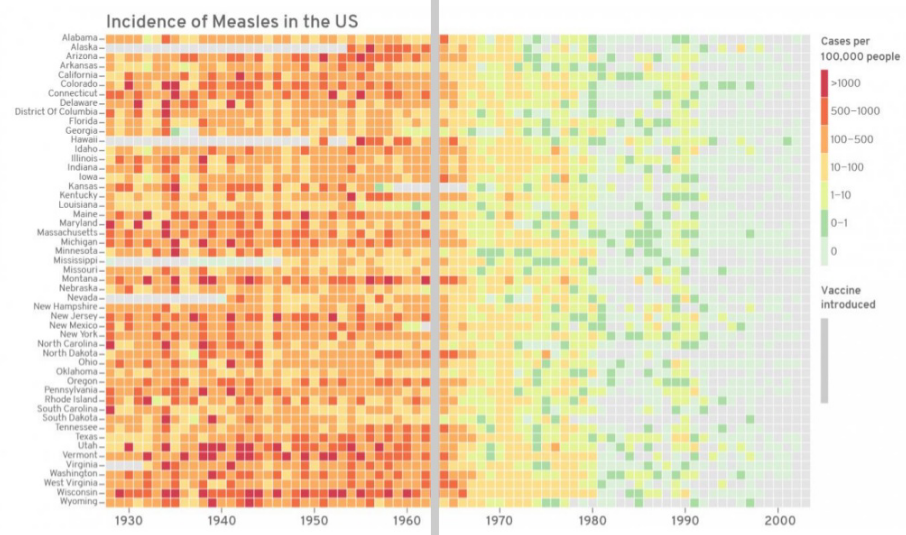
\includegraphics[width=0.7\linewidth]{imgs datavis/Vaccino.png}
	\caption{Incidence of Measles in the US}
	\label{fig:Measles}
\end{figure} 

Per ogni riga vi sono gli stati degli Stati Uniti. I quadrati hanno una dimensione omogenea ed indicano gli anni. Il colore invece indica l'incidenza del morbillo, il rosso indica la presenza di più di mille casi, fino al colore verdino 0 casi. Il colore grigio invece indica assenza di informazioni. Linea grigia verticale: indica l'introduzione del vaccino contro al morbillo (primi anni '60).

Qui vi è una chiara rappresentazione del fatto che intorno agli anni '60 (magari per una tendenza anche precedente all'introduzione del vaccino) si riduce l'incidenza del morbillo nella popolazione americana e negli anni 80 è quasi debellata. In realtà l'introduzione del vaccino non è importante di per sè. Molto importante invece è la penetrazione del vaccino all'interno della popolazione, il fatto che ci sia una campagna vaccinale che aumenta il numero dei vaccini effettuati, poiché ci può essere anche il vaccino ma se i soggetti vaccinati sono pochi la riduzione dell'incidenza della malattia non è certamente associabile all'introduzione del vaccino. Questa visualizzazione come sempre richiede un'interpretazione del contesto. Può essere utilizzata per manipolare l'opinione pubblica, è molto persuasiva. 
Dalle opinioni passiamo alle decisioni. Se effettivamente c'è qualcosa che riguarda la salute siamo nell'ambito tipico delle decisioni. 

\subsection{Where should you get visited}
Ipotizziamo il caso in cui sia necessario effettuare un'operazione al ginocchio e il medico non sia in grado di dare un'opinione sull'ospedale migliore. 

Nello specifico in Lombardia c'è un portale in cui vengono riportate una serie di statistiche sulla performance sanitaria.

\begin{figure}[h]
	\centering
	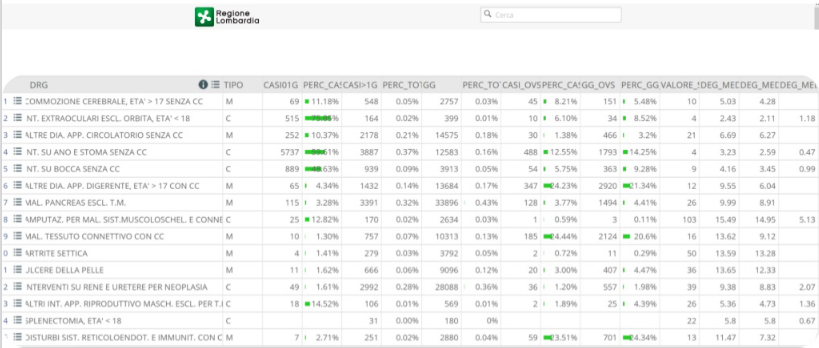
\includegraphics[width=0.5\linewidth]{imgs datavis/Dati Lombardia.png}
	\caption{}
	\label{fig:lombardia}
\end{figure} 

La tabella riporta la qualità delle prestazioni di cura per la cura ai problemi al ginocchio. Tuttavia questa modo di riportare i dati non permette al soggetto di comprendere in modo chiaro l'informazione. 

Da questi dati è stata effettuata la info grafica \ref{fig:esperienza strutture ospedaliere Lombardia} in cui nelle ascisse troviamo il numero di ricoveri, mentre nelle ordinate la percentuale di secondi ricoveri. Il numero di ricoveri indica l'esperienza dei chirurghi in quella struttura, maggiori sono i ricoveri maggiore sarà l'esperienza e viceversa. Nelle ordinate vi è una valutazione degli eventi avversi, qual è la proporzione di interventi che richiedono un secondo intervento, in particolare è considerato secondo ricovero una seconda operazione avvenuta entro 40/50 giorni dalla prima. Ciò significa che il primo non è stato risolutivo oppure sono emersi eventi avversi.  Più un punto si trova in alto peggio è, perché è molto frequente che accadano complicanze. Se la percentuale fosse intorno al 90/100\% dovrebbe essere chiusa la struttura, se invece la percentuale è bassa, intorno al 10\% è piuttosto raro che succedano cose per cui è necessario un secondo intervento.  

Ogni cerchio è un punto dato, è una struttura caratterizzata percentuale media di secondi ricoveri e da numero di ricoveri. Vi sono strutture che fanno pochi interventi di quel tipo e che vanno male (in alto a sinistra). Così come ci sono strutture che effettuano pochi interventi ma presentano un tasso di complicanza basso. 

\`E ovviamente molto importante il combinato di entrambe le dimensioni (media secondi ricoveri e numero di ricoveri) tuttavia tra le due pesa maggiormente il numero di ricoveri, quindi bisognerebbe considerare strutture che effettuano molti interventi (numero di ricoveri). Quello che sembra più ottimale è l'istituto Galeazzi che presenta un numero di ricoveri alto (6000) e una percentuale di secondi ricoveri pari al 40\%.

\begin{figure}[h]
	\centering
	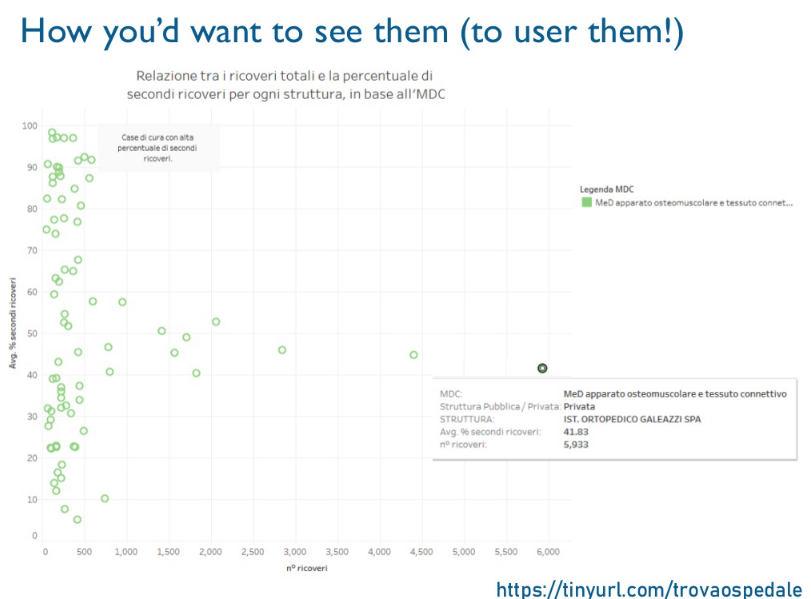
\includegraphics[width=0.4\linewidth]{imgs datavis/Ospedali.png}
	\caption{}
	\label{fig:esperienza strutture ospedaliere Lombardia}
\end{figure} 

Tuttavia, il numero di ricoveri non è sempre un numero fedele dell'esperienza, può accadere infatti che sia un solo chirurgo a effettuare quei ricoveri, pertanto nonostante il numero di ricoveri sia basso il chirurgo sarebbe molto esperto e andare da lui sarebbe una buona scelta. Per ovviare a questo problema ed essere più precisi si potrebbe indicare il numero di ricoveri per chirurgo.

Inoltre, non necessariamente un alto tasso di secondi ricoveri implica bassa esperienza, poiché è probabile che nei migliori centri ospedalieri arrivino casi gravi da ogni parte d'Italia e pertanto si rende necessario un secondo ricovero. 

Non c'è il rischio di manipolare la discussione utilizzando solo i parametri che ho scelto e tralasciandone altri? 

Ovviamente si e questo è uno dei motivi per cui da una parte la visualizzazione da un punto di vista comunicativo, persuasivo può essere efficace e dall'altra essere manipolatrice perché possiamo mostrare alcune cose e non altre e lasciando l'idea che queste ultime non esistano.

\subsection{Covid-19}
La seguente tabella mostra il numero di contagi, di ricoveri in terapia intensiva, ecc. 

Il modo in cui divulghiamo i dati ha un'influenza sui dati stessi poiché comunicare dei dati comporta la costruzione di determinate idee, queste ultime influenzano il loro comportamento e nuovamente i dati.

Come noi andiamo a divulgare i dati e a proporre  gli stessi alla popolazione che prende decisioni tutti i giorni, ha un'influenza sui dati stessi. 
\begin{figure}[h]
	\centering
	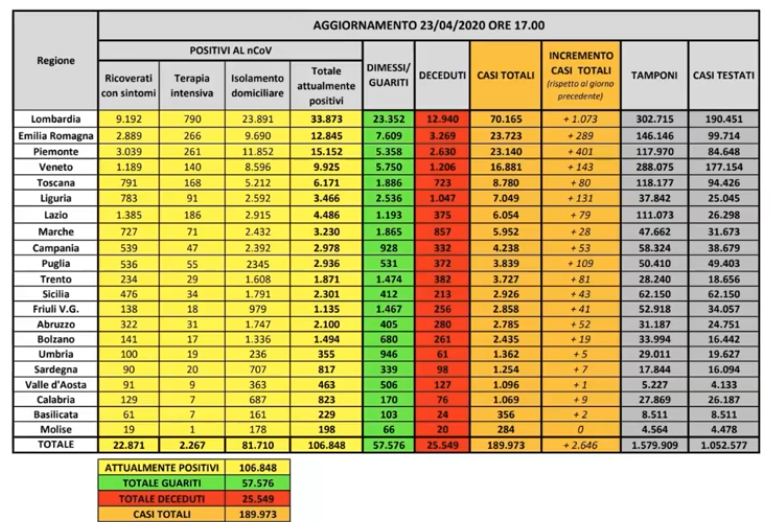
\includegraphics[width=0.6\linewidth]{imgs datavis/Tabella contagi covid-19.png}
	\caption{}
	\label{fig:contagi}
\end{figure} 

\newpage

La figura \ref{fig:contagi1} rappresenta con un grafico ad area proporzionale il numero di contagi da Covid-19. 

\begin{figure}[h]
	\centering
	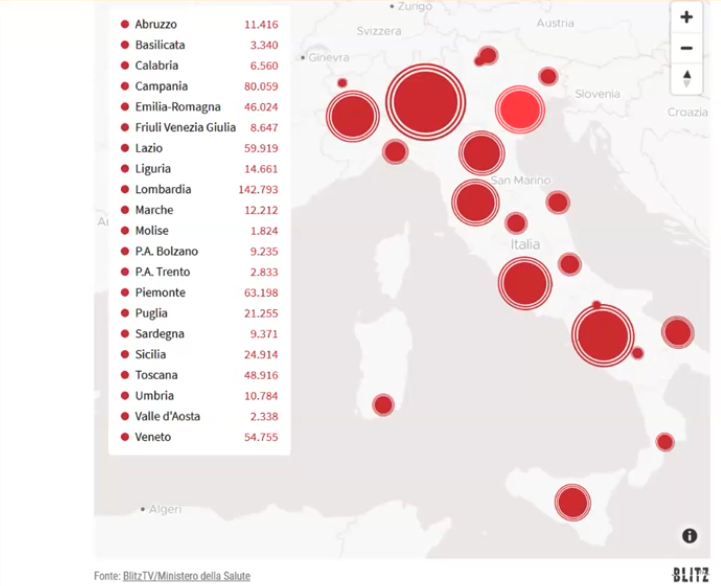
\includegraphics[width=0.6\linewidth]{imgs datavis/Contagi regioni.png}
	\caption{}
	\label{fig:contagi1}
\end{figure} 

Questa rappresentazione pone nel capoluogo di regione o di provincia il centro di questi cerchi e in maniera proporzionale al cerchio rappresenta il numero di casi. \`E molto imprecisa e fuorviante, sembra che tra Milano e Venezia non ci siano casi, ci dà una rappresentazione a granularità molto larga perché se andassimo a confrontare Milano con Bergamo i due cerchi si sovrapporrebbero. 

Una visualizzazione migliore è la \ref{fig:contagi1} dove la granularità è più fine, si lavora sulla tinta e sulla quantità di bianco. 

\begin{figure}[h]
	\centering
	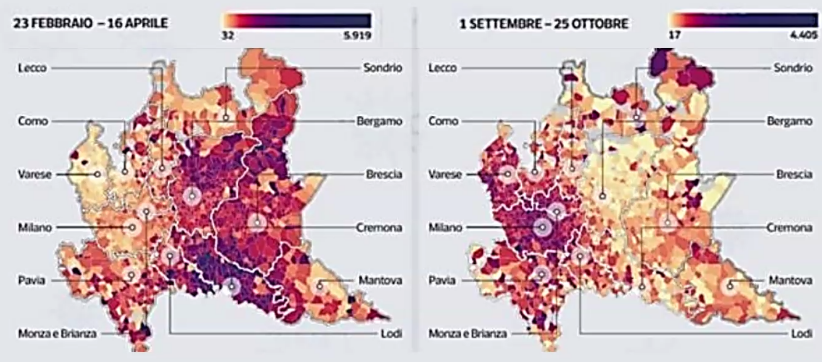
\includegraphics[width=0.6\linewidth]{imgs datavis/Grafico covid Lombardia.png}
	\caption{}
	\label{fig:contagi2}
\end{figure} 

Due visualizzazioni molto simili invitano ad un confronto. \`E possibile vedere l'incidenza tra il 23 Febbraio e il 16 Aprile e tra il 1 Settembre e il 25 Ottobre. Più scuro è il colore maggiore è l'incidenza anche se sarebbe stato meglio normalizzare per il numero di abitanti. Tra la primavera e l'autunno la nuvola nera si sposta da Bergamo/Brescia/Cremona a Milano/Varese. Questa visualizzazione ci consente di valutare se c'è stato un miglioramento, ci consente di capire la dimensione diacronica, cioè se le cose sono migliorate da una parte per peggiorare da un'altra (ciò che effettivamente è successo). 

Nel grafico \ref{fig:contagi3} viene effettuato un confronto fra la Norvegia e la Svezia. Vengono riportati i casi per milione di abitati, quindi i contagi vengono normalizzati per la popolazione (fondamentale).
\begin{figure}[h]
	\centering
	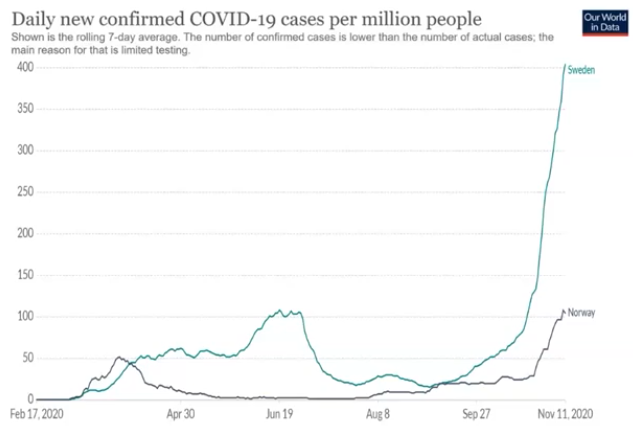
\includegraphics[width=0.6\linewidth]{imgs datavis/Covid2.png}
	\caption{}
	\label{fig:contagi3}
\end{figure} 

Dal grafico si può notare la differenza nella gestione della pandemia nel modello svedese e nel modello norvegese. Inoltre questo grafico riporta la media del numero di positivi nei 7 giorni precedenti, questo significa che si è ammorbidita l'influenza della variazione nella fluttuazione di tamponi fatti. Il difetto deriva da una mancanza di informazioni relative al numero di tamponi. Inoltre non viene specificato il tipo di tampone che viene effettuato.

Ciò che possiamo notare è un aumento esponenziale dei contagi tra Svezia e Norvegia.

Anche questa è una visualizzazione è un po' piatta poiché non hanno una popolazione simile, tuttavia hanno dei modelli di gestione della pandemia diversi pertanto il confronto risulta interessante. 

Il grafico \ref{fig:contagi4} sembra molto più interessante, si cerca di comprendere i fattori latenti nelle varie differenze di derivata.Nei commenti si riporta la reazione dei governanti della Svezia e la reazione della controparte norvegese. Nel vedere tutte le reazioni dei negazionisti, dei governanti, ecc. si comprendono gli andamenti. Nel momento in cui un governo impone la quarantena il numero cala, nel momento in cui ci sono delle politiche più liberali i contagi salgono.

\begin{figure} [h]
	\centering
	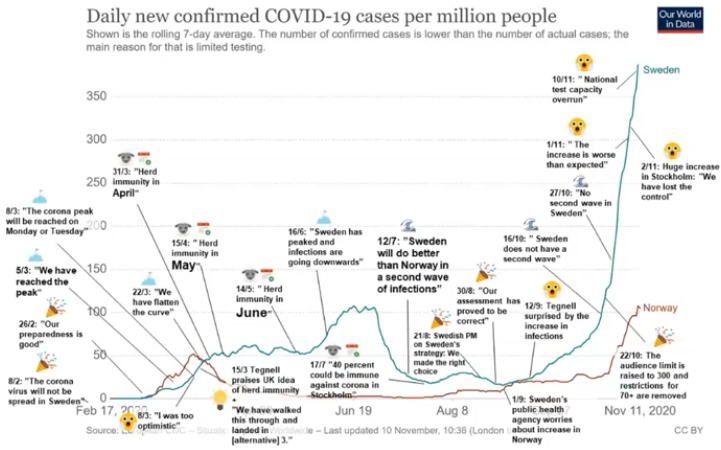
\includegraphics[width=0.6\linewidth]{imgs datavis/Covid3.png}
	\caption{Daily new confirmed COVID-19 cases per million people: Sweden, Norway}
	\label{fig:contagi4}
\end{figure} 


\begin{figure} [h]
	\centering
	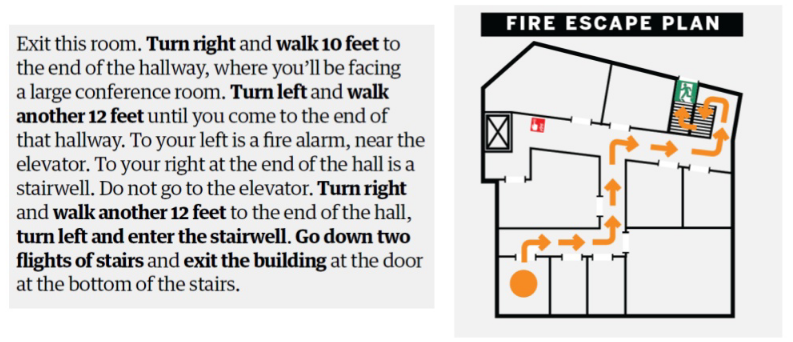
\includegraphics[width=0.6\linewidth]{imgs datavis/esperimento.png}
	\caption{}
	\label{fig:esperimento}
\end{figure} 

\`E stato calcolato che una figura è meglio di 60.000 parole. Una ricerca di psicologia cognitiva ha calcolato che le cose visuali vengono elaborate dal nostro cervello 60.000 volte più veloce di quelle scritte. Siamo inoltre veloci più del doppio a comprendere un'immagine piuttosto che una parola, 10 volte più bravi a recepire un'informazione che ci viene erogata in maniera visuale piuttosto che un'informazione testuale. 

\subsection{Data science and Data visualization: similarities}

Il modo di operare di chi fa scienza con i dati deve essere molto simile a chi fa visualizzazione con i dati. 

\begin{figure}[h]
	\centering
	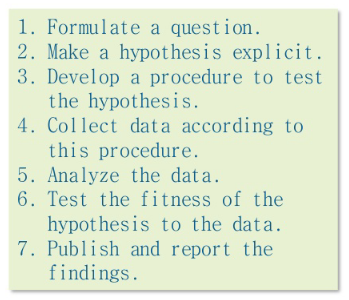
\includegraphics[width=.48\textwidth]{imgs datavis/Passaggi1.png}\hfil
	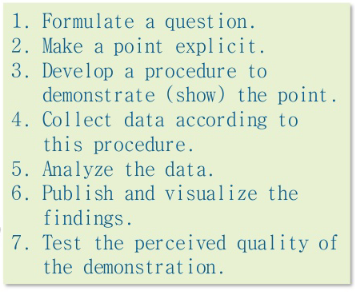
\includegraphics[width=.49\textwidth]{imgs datavis/Passaggi2.png}
	
	\caption{Data Science vs Data visualization}\label{etichetta}
\end{figure}

7. Test the perceived quality of the demonstration: anche noi dovremo testare il nostro modo di provare la tesi ossia la visualizzazione. Dobbiamo tornare dal fruitore della visualizzazione e capire se il vero messaggio è stato trasmesso con quel grafico, se l'obiettivo è stato raggiunto. 

Il data scientist nella visualizzazione non deve essere troppo creativo, dall'altra parte chi avrà necessità di comunicare attraverso le visualizzazioni dovrà cambiare atteggiamento rispetto a chi fa un info grafica semplicemente bella, dovrà seguire un processo mentale con il quale sviluppa la visualizzazione che dovrà essere di qualità. 


\subsection{From data charts to data visualization}

Vi è una differenza fra un data chart ed una visualizzazione. 

\begin{figure}[h]
	\centering
	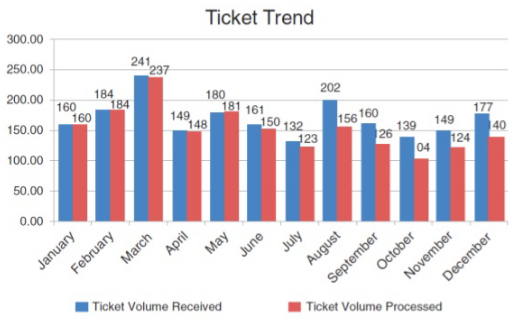
\includegraphics[width=.6\textwidth]{imgs datavis/bar charts.png}\hfil
	
	\caption{Bar chart}\label{etichetta}
\end{figure}


Questo grafico può essere generato facilmente attraverso una procedura wizard (passo passo) di un comune foglio di calcolo: selezione delle colonne, definizione dei riferimenti temporali e scelta del grafico.
Bisogna però capire se questo grafico sia efficace ed efficiente e se abbia tutta una serie di qualità non funzionali legate alla soddisfazione di chi fruisce della visualizzazione. L'efficacia e l'efficienza riguardano invece la leggibilità e la comprensibilità. Analizzando il grafico possiamo vedere che sia la legenda che il titolo ci spiegano di cosa si tratta: si confronta il numero di ticket entrati in un sistema di gestione delle segnalazioni (blu) e il numero di ticket processati (rosso). Si nota una serie temporale indicata con delle categorie mensili. Per ogni mese ci sono due bar chart.  

I software con i quali è possibile fare questo grafico si limitano a fare chart, non visualizzazioni, e la differenza è semantica (difficile da colmare). Noi vogliamo andare oltre e arrivare a questo: 
\begin{figure}[h]
	\centering
	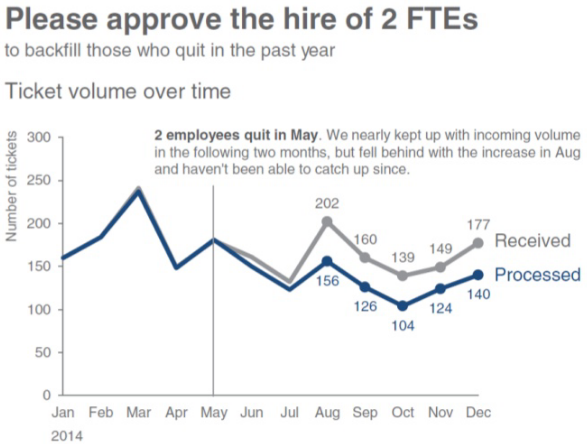
\includegraphics[width=.6\textwidth]{imgs datavis/visualization.png}\hfil
	
	\caption{Correct visualization}\label{Bar chart}
\end{figure}


La data visualization dimostra subito il point ossia la tesi. La tesi della seguente visualizzazione è che c'è un problema Maggio, c'è inoltre una diagnosi route cause analysis, cioè si identifica come causa di una differenza sempre crescente tra ticket in ingresso e ticket in uscita, il fatto che due dipendenti si siano licenziati, quindi si è ridotta la risorsa umana che gestisce i ticket. A partire da maggio vi è una sorta di forbice, ossia la differenza è tale per cui la vediamo anche su una visualizzazione diacronica di una serie temporale. Per le serie temporale è più indicata una linea non delle barre. Questa rappresenta una visualizzazione di qualità che i software non sono ancora in grado di sviluppare. I software non sono in grado di stabilire quanto l'output differisce dall'input. L'essere umano invece capisce il messaggio dietro ai dati. 

Anche la differenza può essere rappresentata in molti modi diversi (in termini assoluti, in percentuale rispetto alla media, ecc. oppure in termini di z-score cioè  quanto i dati variano intorno alla media).

\begin{figure}[h]
	\centering
	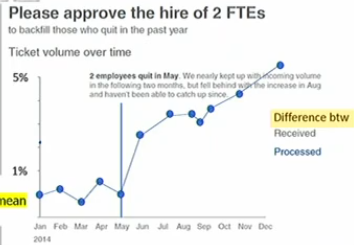
\includegraphics[width=.6\textwidth]{imgs datavis/differenza.png}\hfil
	
	\caption{Difference between tickets}\label{Difference}
\end{figure}

Questi ultimi due grafici possono essere presentati insieme. In tal caso l'informazione sarà più completa.

Visualizzazione: strumento visuale più adeguato per dimostrare una tesi.  

Quando le categorie sono molte l'areogramma non è il chart da scegliere (meglio il bar chart). 

Viene fatta una domanda prima e dopo un seminario. La domanda è la seguente: Quanto ritieni interessante intraprendere un percorso nel quale devi cimentarti in esperimenti scientifici. 


\begin{figure}[h]
	\centering
	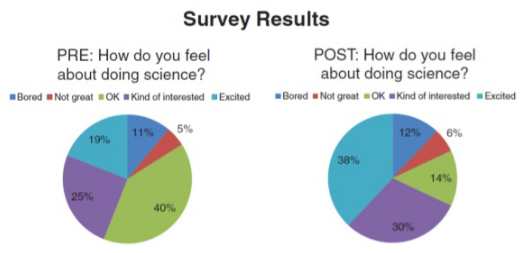
\includegraphics[width=.6\textwidth]{imgs datavis/seminario.png}\hfil
	
	\caption{}\label{}
\end{figure}

Ci sono diverse categorie. Le due rappresentazioni dimostrano quanto è stata efficace la presentazione nello scatenare interesse. Altri prenderebbero queste categorie che sono ordinali (da noioso a interessato) le ordinerebbero e potrebbero calcolarne la media per individuare quanto cambia la media dei dati precedenti e successivi al seminario.

Una differente rappresentazione è quella che utilizza le barre (le barre non sono negative in sè).


\begin{figure} [h]
	\centering
	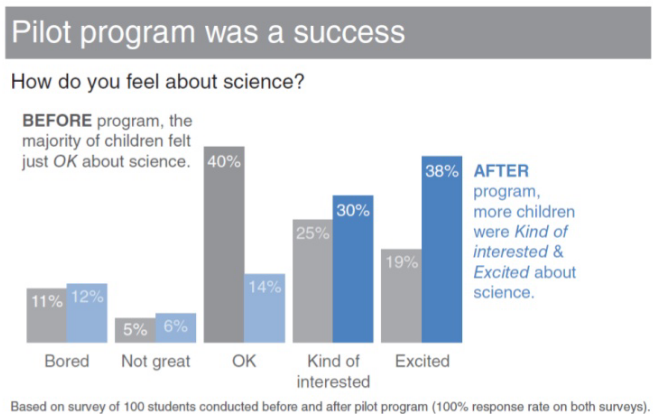
\includegraphics[width=.6\textwidth]{imgs datavis/seminario 1.png}\hfil
	
	\caption{}\label{}
\end{figure}

 Quest'ultima ci mostra una piccola differenza nella categoria annoiato, così come possiamo vedere che la categoria OK presenta prima molti soggetti indecisi, successivamente rimane solo un 14\%, vediamo un aumento del 5\% sulla penultima categoria e un aumento del doppio sull'ultima categoria. Un altro elemento che differenzia un chart da una visualizzazione è il context 


\begin{figure}[h]
	\centering
	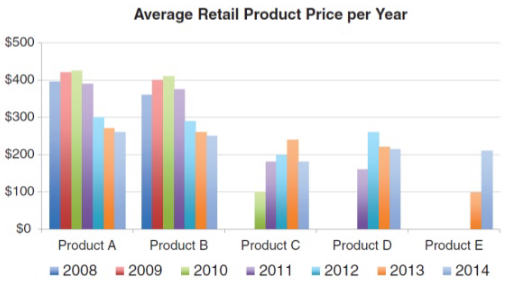
\includegraphics[width=.6\textwidth]{imgs datavis/prezzi prodotti .png}\hfil
	
	\caption{}\label{}
\end{figure}
Diversi anni = diversi colori 

Diversi been = diversi prodotti 

Le barre indicano l'evoluzione del prezzo di un certo prodotto, l'informazione oltre che posizionale (sull'anno) viene erogata anche in maniera cromatica (ridondanza). E' questo l'obiettivo? Questa visualizzazione non sembra dimostrare la tesi.

La seguente visualizzazione sembra più utile:


\begin{figure}[h]
	\centering
	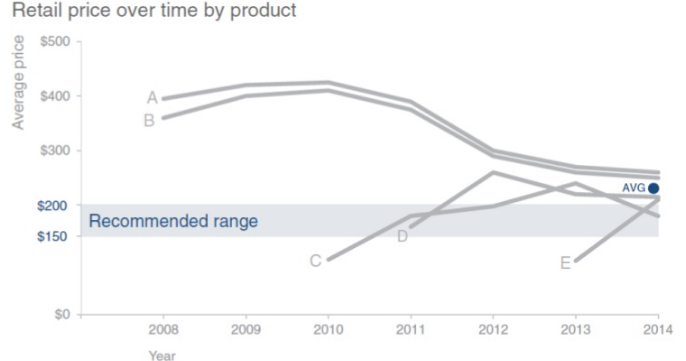
\includegraphics[width=.6\textwidth]{imgs datavis/prezzi prodotti 1.png}\hfil
	
	\caption{}\label{}
\end{figure}

Ha una sua funzione, cerca di dimostrare qualcosa. C'è infatti un range raccomandato e tendenzialmente i prodotti vi convergono nel tempo, quindi c'è un prezzo giusto da proporre alla clientela, questo è autoesplicativo nel momento in cui si mostrano i dati nel modo corretto.

Nel seguente grafico, vediamo un elevato numero di categorie, forte indizio che deve essere sostituito da un'altra visualizzazione. 

\begin{figure} [h]
	\centering
	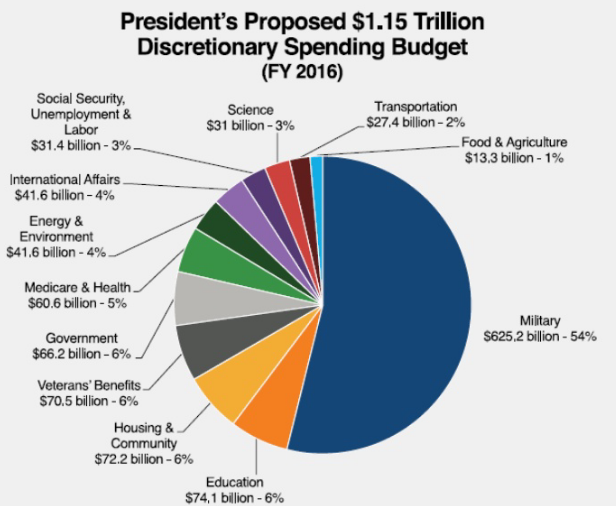
\includegraphics[width=.48\textwidth]{imgs datavis/spese.png}\hfil
	
	\caption{}\label{}
\end{figure}

In questo caso vediamo come il budget degli stati uniti venga proposto di essere diviso. Si può notare che più del 50\% venga dedicato alle spese militari. Quando l'areogramma ci facilita la lettura dei rapporti è adeguato. Diventa tuttavia difficile capire se il budget dedicato ai veterani sia più grande rispetto al budget dedicato al governo. Quando gli spicchi diventano molto stretti diventa difficile effettuare confronti. E' quindi un chart che può essere generato molto facilmente. 

La seguente invece è la stessa visualizzazione in uno stacked bar chart che rinuncia a far capire perfettamente come il budget venga diviso, ma ritiene che alcune spese debbano essere aggregate.

\begin{figure}[h]
	\centering
	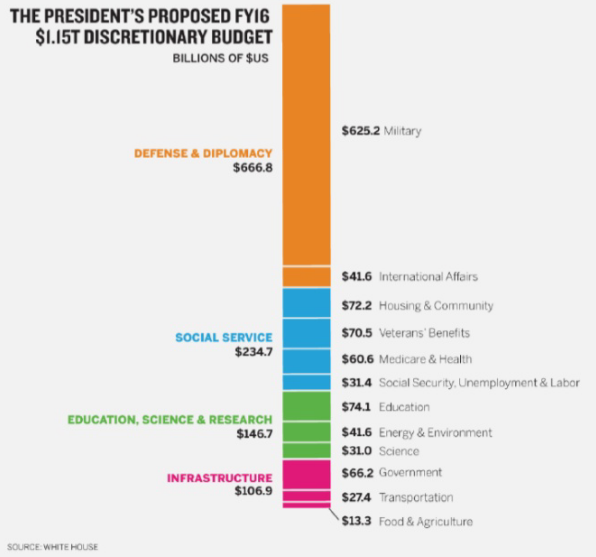
\includegraphics[width=.48\textwidth]{imgs datavis/Budget.png}\hfil
	
	\caption{}\label{}
\end{figure}

 In questo modo si crea una narrativa. Si è scoperto che il modo migliore per raccontare qualcosa a qualcuno è quello di metterla dentro una storia. Questo è un primo modo per raccontare qualcosa.    

\newpage
Qui viene mostrato il prezzo di una birra in diversi stadi. 
\begin{figure}[h]
	\centering
	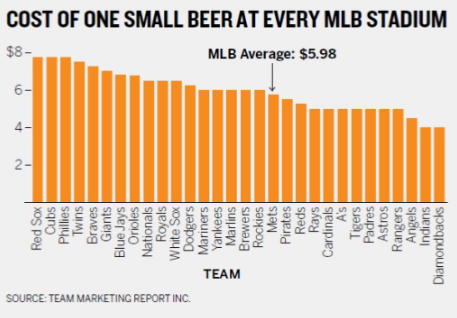
\includegraphics[width=.58\textwidth]{imgs datavis/prezzi birra.png}\hfil
	
	\caption{}\label{birra}
\end{figure}

Per ogni stadio viene rappresentato il costo con una birra. L'ultimo stadio è quello in cui troviamo la birra meno costosa. 

\newpage
Questo è un altro modo di visualizzare i dati. 
\begin{figure}[h]
	\centering
	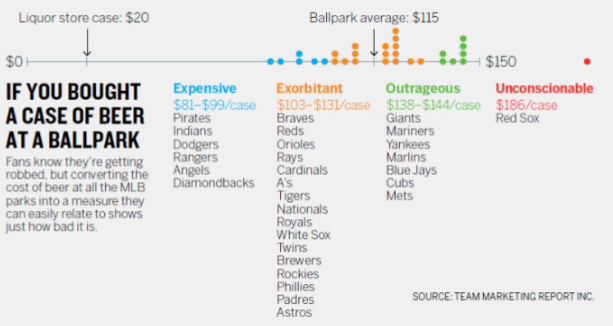
\includegraphics[width=0.40\textwidth]{imgs datavis/prezzi birra 1.png}\hfil
	
	\caption{}\label{}
\end{figure}

In questo caso il punto di vista di chi l'ha fatto si esplica anche nelle etichette messe alle diverse porzioni di dati. Lui sceglie di aggregare diversi prezzi e di caratterizzarli con costoso, esorbitante, oltraggioso, inconcepibile. Questa visualizzazione ci consente di capire in quanti stadi la birra ha lo stesso prezzo. Viene anche visualizzata la media. 

La differenza fra i due grafici è che, con gli stessi dati, a livello di efficacia argomentativa nel secondo vi è un contesto che racconta una storia. 

\subsubsection{Field of view and point of view}

Due concetti sono estremamente importanti nella visualizzazione: campo visuale e punto di vista. 

\paragraph{Field of view}

\begin{figure}[h]
	\centering
	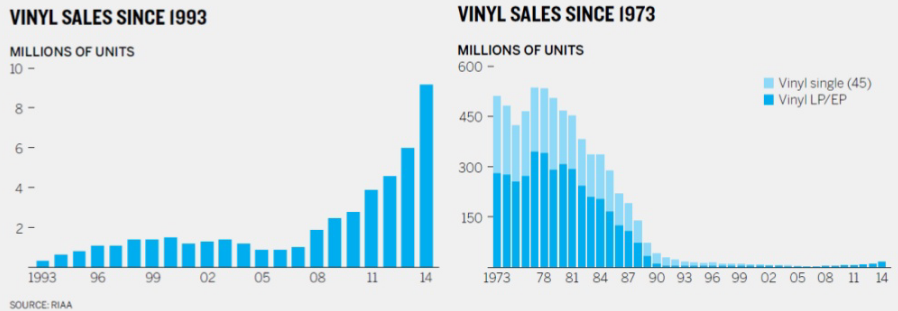
\includegraphics[width=.4\textwidth]{imgs datavis/vinili.png}\hfil
	
	\caption{}\label{}
\end{figure}

Quantità di dischi in vinile venduti dal 1993 al 2014. Un aumento di dieci volte. Il vinile sta tornando? In realtà se si cambia il campo visuale includendo ulteriori 20 anni vediamo come in realtà cambia l'intero giudizio e la storia che possiamo raccontare è diversa. E' vero che c'è stato un aumento ma questo non è comparabile ai dischi venduti nel ventennio tra il 1973 e il 1993. 

Field of view: è possibile raccontare due storie diverse. 
\paragraph{Point of view}
Quale asset è più volatile? 
\begin{figure}[h]
	\centering
	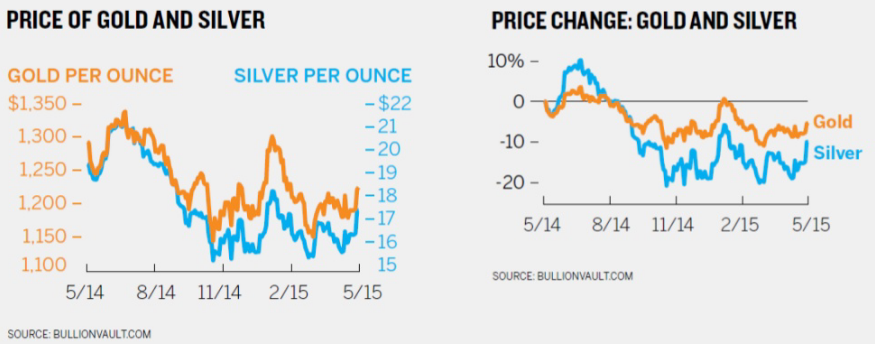
\includegraphics[width=.48\textwidth]{imgs datavis/oro vs argento.png}\hfil
	
	\caption{}\label{}
\end{figure}

Dal primo grafico sembrerebbe che l'oro sia più volatile dell'argento, tuttavia guardando il secondo grafico che mostra la variazione percentuale mostra invece che l'argento subisca maggiori variazioni rispetto all'oro. Con gli stessi dati, solo cambiando il punto di vista è possibile trarre conclusioni diverse. 

Point of view: è possibile raccontare una storia che può essere travisata completamente. 

\begin{figure}[h]
	\centering
	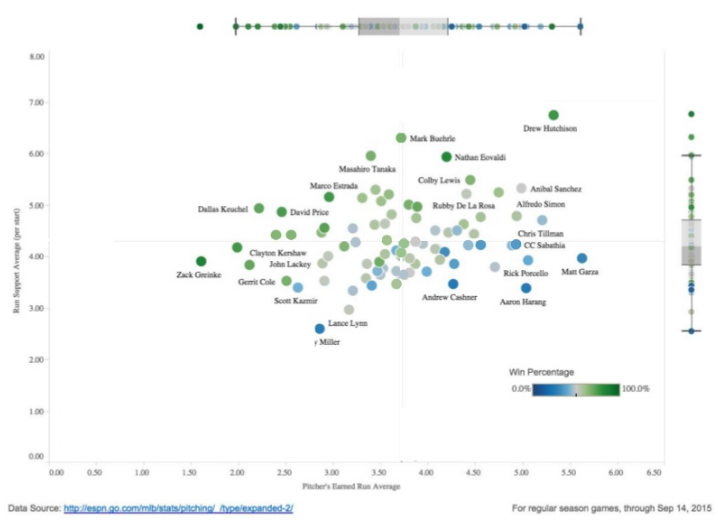
\includegraphics[width=.5\textwidth]{imgs datavis/scatter plot.png}\hfil
	
	\caption{}\label{}
\end{figure}

In questa immagine vengono divisi i giocatori bravi-fortunati, bravi-sfortunati, cattivi-fortunati e cattivi-sfortunati. Bravo se segna, fortunato se si trova in una squadra che vince. 

Importanti anche i box-plot.

Lo scatter plot permette di rappresentare le diverse fasce di normalità che però non coincidono con la proiezione del box plot poiché quest'ultimo rappresenta il range interquartile, la fascia di normalità si compone partendo dalla mediana e non dalla media e costruendo una fascia ampia due sigma. Tutti i punti all'interno dell'intersezione fra queste due bande sono punti normali, tutti quelli fuori sono punti notevoli che devono essere considerati. 

\begin{figure}[h]
	\centering
	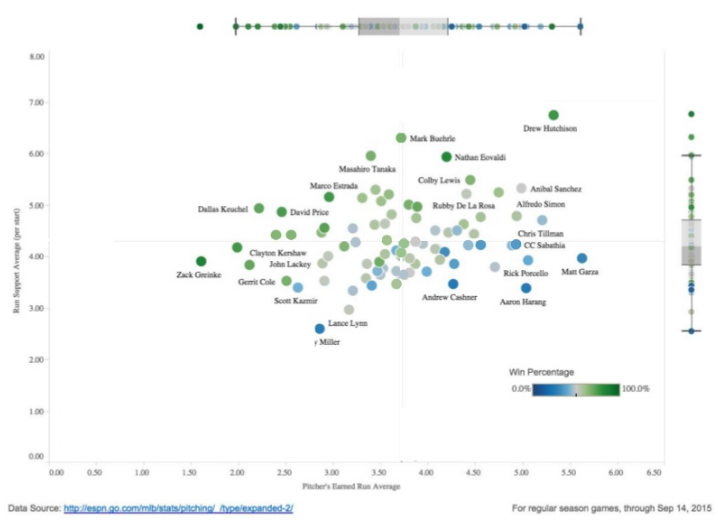
\includegraphics[width=.5\textwidth]{imgs datavis/scatter plot.png}\hfil
	
	\caption{}\label{scatter plot}
\end{figure}

Gli stessi dati possono essere distribuiti in modo diversi, anche se caratterizzati da stessa media. Possono essere simmetrici, possono avere degli outliers, possono essere bimodali, possono avere cardinalità diverse per esempio nel caso di confronti di medie. 


\begin{figure}[h]
	\centering
	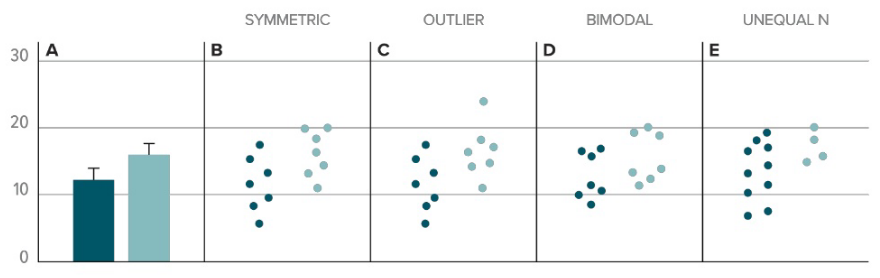
\includegraphics[width=.5\textwidth]{imgs datavis/media.png}\hfil
	
	\caption{}\label{}
\end{figure}


Dot plot apprezzabile perché fa vedere i singoli punti che caratterizzano una distribuzione, dà un'idea della varianza e come si distribuiscono nell'intero range, se ci sono outliers e se ci sono più mode. Non fare vedere i punti che corrispondono ai dati ci impedisce di vedere cose che invece potrebbero essere interessanti e che potrebbero anche essere molto fuorvianti. Nella \ref{scatter plot} possiamo vedere: a sinistra che il data set azzurrino ha una media superiore rispetto al data set più scuro. In realtà i data set hanno delle proprietà che possono rendere la media un parametro poco significativo: per esempio possono essere simmetrici, presentare outliers, le distribuzioni potrebbero presentare più mode oppure ci potrebbero essere forti differenze a livello di numerosità del campione (cardinalità). 

Nella data visualization dovremmo ragionare per sottrazione: far vedere tutti i dati, se però questo è troppo magari risulta più utile evidenziare solo alcuni parametri. 

I dotplot hanno la caratteristica di mostrare i punti-dato il che risulta interessante quando la loro distribuzione è significativa. Il grafico (dot plot mettere riferimento,) mostra la relazione fra la dose del farmaco e la permanenza in ospedale. Violin box-plot migliore del normale box-plot perché presenta anche una forma.


 \begin{figure}[h]
 	\centering
 	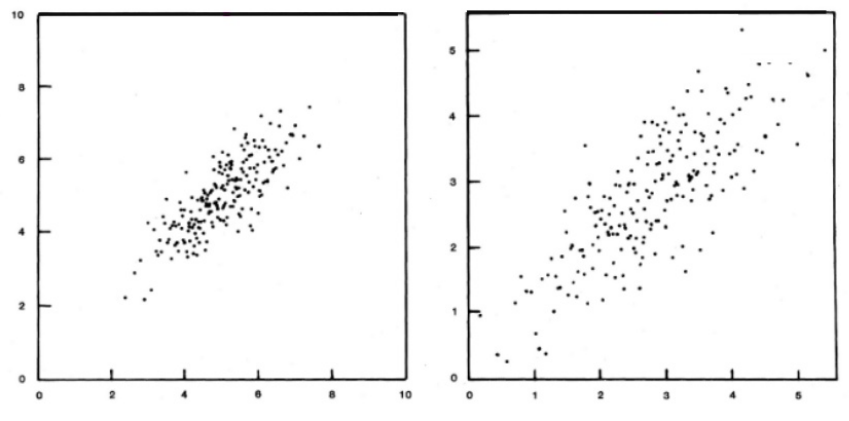
\includegraphics[width=.5\textwidth]{imgs datavis/double scatter.png}\hfil
 	
 	\caption{}\label{}
 \end{figure}

Anche gli scatter plot presentano dei problemi. 

Quale dei due presentano dati più correlati? La maggior parte dei soggetti ritiene che lo scatter plot di sinistra presenti dati più correlati. In realtà entrambi hanno medesima correlazione. 

In ambito bio informatico e bio medico si usano diagrammi come il seguente:

\begin{figure}[h]
	\centering
	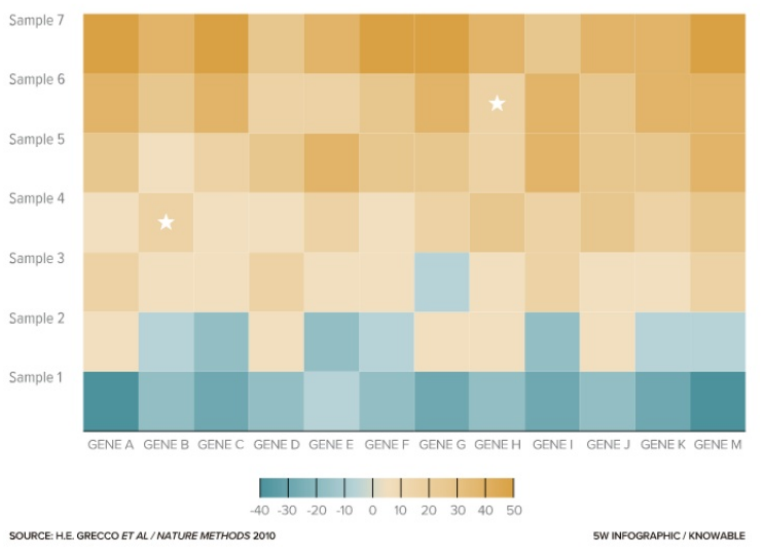
\includegraphics[width=.58\textwidth]{imgs datavis/quadri .png}\hfil
	
	\caption{}\label{}
\end{figure}

Questo diagramma indica la presenza in un diagramma campione biologico. Con questo grafico si voleva mostrare come il gene b e il gene h fossero presenti in egual misura nel campione 4 e nel campione 6. Un soggetto che osserva questo grafico potrebbe essere tratto in inganno e pensare che il gene b sia maggiormente presente nel campione 4 rispetto al gene h nel campione 6, in realtà quei geni sono presenti nella stessa misura nei 2 campioni, si tratta semplicemente di un'illusione ottico-cromatica.

\subsection{Four myths on data visualization}
\subsubsection{Data visualization is simple. You just need to insert a chart}

Vi sono moltissimi modi per sbagliare una visualizzazione i dati. Una recente indagine ha individuato che ben 8 grafici su 10 pubblicati (per esempio in riviste) presentano qualche errore che distorce o ha la potenzialità di distorcere il messaggio che chi l'ha messa vuole veicolare. Questo può avvenire: per incompetenza (manca sensibilità, consapevolezza e cultura della grafica) o in modo volontario.

Per esempio un articolo mostra attraverso dei cerchi la quota di investimenti, tuttavia i cerchi non corrispondono alla reale quota dell'investimento. C'è un errore di 100 volte.

Grafici a torta: molti potrebbero essere tentati a dare originalità introducendo la terza dimensione. la terza dimensione potrebbe essere utile quando si devono rappresentare tre variabili. In tutti gli altri casi andrebbe evitato. Nel grafico seguente potremmo chiederci se il prodotto D vende di più del prodotto B. Dal grafico a sinistra sembrerebbe di si, tuttavia se andassimo a guardare il secondo grafico senza la terza dimensione vedremmo che entrambi i prodotti vendono pari quantità. 

Mappe coropletiche: mappa che colora alcune aree in un certo modo in funzione di una variabile di interesse. In questo caso abbiamo una variabile dicotomica (rosso repubblicano, blu democratico). Qui vengono rappresentati i voti repubblicani e democratici per capire chi aveva vinto nelle elezioni presidenziali americane. A livello di stati Trump vinse molto, soprattutto vinse a livello di contea. Nel grafico in alto a destra sembra che tale vittoria fu schiacciante, questo perché la densità di popolazione degli stati uniti è eterogenea, la maggior parte si distribuisce nelle coste mentre al centro è molto bassa. Vincere in una contea con pochissimi abitanti non vale quanto vincere in una contea con moltissimi abitanti. 

L'utilizzo di un cartogramma (mappa 3) agisce anziché sul colore sull'estensione del territorio. Quindi in basso vediamo che gli stati più popolosi occupano più spazio nella mappa di quelli meno popolosi. In questo caso vediamo che la quantità di rosso non è molto diversa dalla quantità di blu. Questo perché in termini di voti Clinton ha preso più voti, eppure perse per il sistema elettorale americano. 


Le due figure seguenti che si riferiscono alle attuali elezioni presidenziali americane ci permettono di fare un discorso molto simile. Nella figura in alto che è ancora una volta a livello di contea sembra che tutti abbiano votato per il candidato repubblicano. Se invece guardiamo la figura in basso vediamo che in realtà anche in questo caso i democratici hanno preso molti più voti. 

Quindi il primo mito, ossia fare le visualizzazioni è semplice è falso perchè in realtà la probabilità di fare un errore è molto alta. 

\subsubsection{Data visualization is just a fad. Soon nobody will care}

Mito falso: la visualizzazione dei dati è di più di 300 anni fa, forte necessità di visualizzare i dati a partire dalla nascita degli stati nazionali, cioè con l'insorgere dell'esigenza della buona gestione delle cose dello stato: scienza della buona amministrazione e del governo. 
 
Link per vedere a quali anni risalgono le visualizzazioni che utilizziamo oggi https://history.infowetrust.com/. 

Noi sentiamo, come società, l'esigenza di visualizzare i dati da quando abbiamo i dati. 

\subsubsection{Visualizing data should be the last thing to do}

Il core dell'attività è cercare i dati, analizzarli, interpretarli e successivamente visualizzarli. Tuttavia abbiamo già detto che la visualizzazione è estremamente importante anche nelle primissime fasi come l'esplorazione. Guardare i dati ancora prima di interpretarli è fondamentale e per farlo è necessario visualizzarli. 


\subsubsection{Data visualization make data pretty, but doesn't bring real value}

La visualizzazione non è un elemento di rappresentazione con un valore estetico ma è un momento in cui noi riusciamo ad utilizzare veramente i dati. Anche nel 1849 i dati delle morti per colera a Londra venivano dati in una  tabella al comitato tecnico scientifico per prendere delle misure. Si parlava di 14.000 morti (62 ogni 10.000 abitanti, il covid ora fa 7 morti ogni 10.000 abitanti). Epidemia quasi 10 volte più mortale di adesso. Un medico inglese è voluto andare oltre e ha voluto rendere il dato maggiormente granulare, con una mappa topografica di Londra è andato a rappresentare su ogni palazzo il numero di bare, così facendo è riuscito a capire che c'erano dei pattern, cioè intorno a certi luoghi il numero di morti era maggiore, arrivando a capire il luogo del focolaio. Quegli stessi grafici verrebbero ora riprodotti con dei grafici ad aree proporzionali o con delle mappe di calore. La visualizzazione gli ha permesso di capire che c'era qualcosa che non andava nella fontanella, infatti era un impianto idrico contaminato da una fogna. Solo grazie alla visualizzazione quel medico riuscì ad isolare la causa del colera, da lì si è innescato un movimento scientifico che ha portato alla nascita della moderna epidemiologia. 

La visualizzazione pertanto non è solo un aspetto estetico ma porta valore alle nostre pratiche di comprensione ed interpretazione della realtà e di intervento su di essa.

La data visualization riguarda la fruizione dei dati, l'uso. 

\subsection{From DV to HDI}
Come si passa dalla data visualization classica alla human data interaction? Ci aiuta la tecnologia digitale. Già con un semplice foglio c'è un'interazione. Nella visualizzazione classica c'è il mondo reale, noi ne possiamo creare una rappresentazione codificata ad esempio numerica, i dati poi vengono trasformati attraverso un linguaggio rendendoli più visivi cioè vengono mandati nel dominio di ciò che è percepibile al cervello umano (visual cues- indizio visuale), l'indizio è ciò che fa scattare il processo interpretativo. Con l'interpretazione si passa al mondo reale. L'esistenza di controlli che ci permettono di modulare come i visual cues ci vengono forniti e noi consumiamo  ci da modo di retro azionare questo canale e quindi di manipolare questi controlli (visual cues). Se ci focalizziamo sull'interazione e vogliamo fare scienza su questo aspetto lo strumento più sviluppato finora è la teoria dei media, in particolare la corrente enattivista (enactivism: nell'interagire coi media noi produciamo i media quanto veniamo prodotti da essi). Se invece ci focalizziamo sulla fase dell'interpretazione allora lo strumento che utilizziamo è la teoria semiotica. 

\subsection{What make a good Inforgraphic?}

Vi sono diverse visualizzazioni che cercano di far capire quali sono i componenti fondamentali per una buona visualizzazione. 

\begin{description}
	\item[Data] 
	\item[Design] Capacità di progettare una visualizzaione
	\item[Story] Bisogna comunicare una storia (tesi, point)
	\item [Shareability] Renderlo in un formato condivisibile
\end{description}

\newpage
\section{Good and bad practise for data visualization}

Huff nel ‘54 porta degli esempi di distorsione di messaggi con delle rappresentazioni umoristiche. Entra in gioco il punto di vista: la distorsione cambia la conclusione. 

L'idea è quella di distinguere una distorsione voluta, maliziosa e manipolatoria da una distorsione che è un approccio leggero. 

La volontà fuorviante la si può notare anche guardando il context. 

\begin{figure}[h]
	\centering
	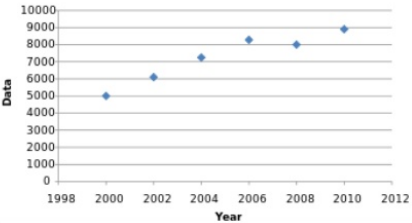
\includegraphics[width=.48\textwidth]{imgs datavis/puntini 1 .png}\hfil
	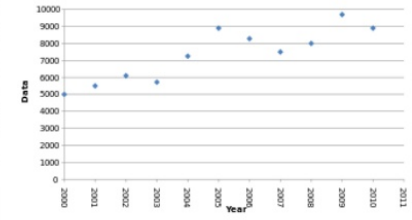
\includegraphics[width=.49\textwidth]{imgs datavis/puntini 2.png}
	
	\caption{}\label{}
\end{figure}

Suggerisce un andamento di crescita costante. Sembra corretto, ma analizzandone gli assi notiamo che nello sviluppo temporale sull'asse X gli intervalli sono di due anni. Analizzando lo stesso grafico aumentando la granularità e prendendo in considerazione tutti gli anni notiamo quello che potrebbe essere un caso di cherry picking, cioè gli anni pari sono stati scelti appositamente per mostrare un messaggio non corrispondente a quello reale.

\begin{figure}[h]
	\centering
	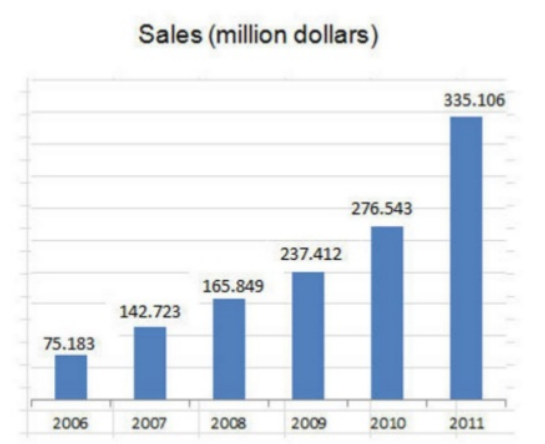
\includegraphics[width=.48\linewidth]{imgs datavis/altezza sprop .png}\hfil
	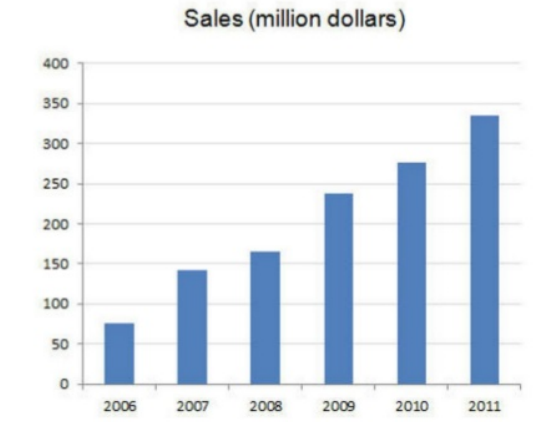
\includegraphics[width=.49\linewidth]{imgs datavis/sprop 2 .png}
	
	\caption{}\label{}
\end{figure}

Quello che sembra un grafico a barre corretto in realtà ha diversi errori:

Manca l’asse verticale che comporta problemi di percezione. La differenza fra le ultime due barre è eccessiva. Un grafico corretto distribuisce le barre in modo diverso. Le differenze si riducono. La manipolazione è intenzionale, difficile fare errori come questo.  


\begin{figure}[h]
	\centering
	\includegraphics[width=0.3\linewidth]{"imgs datavis/linee"}
	\caption{}
	\label{fig:linee}
\end{figure}

\newpage
L’asse Y è ancora una volta il problema, la distanza fra i ‘tick’ da un valore all'altro è distorta e non uniforme. La distanza fra 10.000 è 20.000 è più che proporzionale rispetto alle altre differenze. Anche in questo caso la distorsione è maliziosa e intenzionale.

\begin{figure}[h]
	\centering
	\includegraphics[width=0.4\linewidth]{"imgs datavis/log vs lineare"}
	\caption{}
	\label{fig:log-vs-lineare}
\end{figure}

Qui vediamo la retribuzione oraria di un lavoratore. Possiamo vedere che nel secondario con l'andare del tempo vi è un aumento esponenziale fino ad un picco nel 1975, successivamente il costo comincia a scendere e fluttuare fino a una recente risalita negli anni 2000.

Se rappresentiamo gli stessi dati su scala logaritmica vediamo comunque un andamento crescente tuttavia lineare. Si perdono addirittura certe fluttuazioni negative. 

La scelta della scala lineare o logaritmica dipende dalle intenzioni e di ciò che vogliamo dimostrare. 


Guardando il seguente grafico (sinistra) siamo indotti a pensare che la differenza aumenta sempre ed è massima fra l'ultima barra e la prima. Tuttavia se non troncassimo l'asse vedremmo che in realtà l'aumento è inferiore (grafico a destra). 

\begin{figure}[h]
	\centering
	\includegraphics[width=0.4\linewidth]{"imgs datavis/assi troncati "}
	\caption{}
	\label{fig:assi-troncati-}
\end{figure}

È giusto far partire l’asse verticale da 0 e non ‘zoommare’ sull'asse, perché troncandolo si distorce il messaggio. 

\begin{figure} [h]
	\centering
	\includegraphics[width=0.4\linewidth]{"imgs datavis/colonne rosse e blu"}
	\caption{}
	\label{fig:colonne-rosse-e-blu}
\end{figure}


Anche qui (grafico sinistra) sembra evidente l'intento distorsivo. Se però adottiamo una rappresentazione corretta (grafico destra), non vi è una significativa differenza fra le due squadre. 

\begin{figure}[h]
	\centering
	\includegraphics[width=0.4\linewidth]{"imgs datavis/grafico blu istograffa "}
	\caption{}
	\label{fig:grafico-blu-istograffa-}
\end{figure}


In questo caso non solo il grafico è tagliato ma viene zoomato nell'ordine delle cifre decimali, quindi il tasso di interesse fra il 2008 e il 2012 sembra aumentare esponenzialmente. È possibile argomentare che per chi lavora su cifre ridotte questa visualizzazione sarebbe corretta, ma non avrebbe valore perché non sarebbe utile. Sarebbe opportuno per l’utente non esperto una nota. Attenzione al contesto!

\textbf{Lie factor}: fattore menzogna. E' la dimensione di un effetto come questo è mostrato in un grafico normalizzato (diviso) per la dimensione reale dell'effetto nei dati su cui quel grafico è basato 

\begin{equation}
	LF= \frac{first value - second value}{first value}
\end{equation}

Il rapporto ideale è 1, e comunque compreso nell’intervallo (0.95, 1.05). Non è comunque detto che un valore diverso ci dica che qualcosa è sicuramente una bugia, ma è comunque un indicatore di sproporzione. 

\begin{figure}[h]
	\centering
	\includegraphics[width=0.4\linewidth]{"imgs datavis/pil"}
	\caption{}
	\label{fig:pil}
\end{figure}

A sinistra l'andamento del PIL statunitense da gennaio 2014 a maggio 2015 subisce un tracollo. Tuttavia se andiamo a plottare lo stesso andamento su un grafico dove l'asse non è troncato vediamo che c'è un calo ma non è così cospicuo. 

\begin{figure} [h]
	\centering
	\includegraphics[width=0.4\linewidth]{"imgs datavis/berlusca"}
	\caption{}
	\label{fig:berlusca}
\end{figure}

Questo grafico mostra una decrescita nella fiducia nei confronti del governo Berlusconi. Come possiamo vedere, inizialmente chi era contro era in maggioranza rispetto ai soggetti pro, tuttavia vediamo che anche la fiducia di coloro che avevano sostenuto il governo Berlusconi piano piano decresce. 

Anche in questo caso tagliare l'asse comporta una distorsione, infatti la forbice sembra molto più grande rispetto al caso in cui l'asse parte da 0. 

\begin{figure}[h]
	\centering
	\includegraphics[width=0.5\linewidth]{"imgs datavis/gradi"}
	\caption{}
	\label{fig:gradi}
\end{figure}

Qui vediamo i cambiamenti di temperatura dagli anni 70 al 2005 in un contesto quale quello del cambiamento climatico in relazione all'attività umana. Sembra che non ci siano stati grandi cambiamenti. 

Se andiamo a considerare la differenza e non il valore assoluto, nonostante sia piccola questa si è guadagnata attraverso un aumento monotono. 

Nel grafico blu vi è un fenomeno che potrebbe essere considerato in correlazione al cambiamento climatico ossia la radiazione cosmica, come possiamo vedere sembra vi sia una correlazione negativa, al diminuire della radiazione cosmica c'è un aumento delle temperature. Probabilmente in questo sito si cercava di convincere la gente sull'esistenza di cause esterne all'attività umana. 

È meglio non troncare, ma se ci fosse necessità di utilizzare un asse troncato per notare differenze molto piccole su delle barre si possono visualizzare cosi:

\begin{figure}[h]
	\centering
	\includegraphics[width=0.5\linewidth]{"imgs datavis/teoria "}
	\caption{}
	\label{fig:teoria-}
\end{figure}

Linee guida generali: 
\begin{itemize}
	\item Per il grafico a barre c'è un consenso diffuso che l'asse y non dovrebbe essere troncato; 
	\item Per le linee temporali non c'è un consenso, dipende l'obiettivo che abbiamo, può essere ammesso un troncamento dell'asse y. 
\end{itemize}


\begin{figure}[h]
	\centering
	\includegraphics[width=0.5\linewidth]{"imgs datavis/23"}
	\caption{}
	\label{fig:23}
\end{figure}


Un altro problema non riguarda tanto l'asse tagliato ma quello che noi abbiamo definito scope: se guardo lo stesso incremento nel contesto più generale ridimensiono anche le grandezze in gioco, le differenze in gioco e anche il ragionamento. 

\newpage
Casi di poliomielite tra il 1952 e il 1965:

\begin{figure}[h]
	\centering
	\includegraphics[width=0.5\linewidth]{"imgs datavis/2"}
	\caption{}
	\label{fig:2}
\end{figure}

Il calo sembra iniziare prima dell'introduzione del vaccino (1955), allargando l’attenzione su un grafo più complesso che include una linea temporale più ampia si può notare che c'è stato sì un calo ma come parte di un andamento che ha caratterizzato anche gli anni precedenti. L'introduzione del primo vaccino non sembra abbattere l'incidenza, anche perché dire che è stato introdotto un vaccino non significa necessariamente che è stato somministrato a tutta la popolazione immediatamente. Si può vedere che a partire dal 1961 la malattia scompare. Quindi è possibile sostenere due tesi: la prima secondo la quale il vaccino è stato introdotto in una fase di calo naturale, la seconda secondo la quale il vaccino ha risolto completamente il problema della poliomielite. 

Pertosse 1940-2011

\begin{figure}[h]
	\centering
	\includegraphics[width=0.4\linewidth]{"imgs datavis/12"}
	\caption{}
	\label{fig:12}
\end{figure}


Qui non soltanto si fa vedere il momento in cui è stato introdotto il vaccino ma anche la proporzione di popolazione che si vaccinava. Se non avessimo quest'ultima informazione sembrerebbe che il vaccino non ha diminuito l'incidenza della malattia, tuttavia in corrispondenza dei picchi la popolazione vaccinata era inferiore al 50\%. Quando invece il numero dei vaccinati si assesta intorno al 95\% l'incidenza della malattia è pari a 0. In generale quando si effettua una rappresentazione a doppio asse si sta implicando una qualche correlazione. 


Qui invece vediamo il tasso di decessi per morbillo. 

\begin{figure}[h]
	\centering
	\includegraphics[width=.40\linewidth]{imgs datavis/12a.png}\hfil
	\includegraphics[width=.40\linewidth]{imgs datavis/12b.png}
	
	\caption{}\label{}
\end{figure}


Ancora più forte in questa visualizzazione l'idea che il vaccino non sia riuscito a ridurre i decessi. Nel tempo vediamo che probabilmente per le migliori condizioni igieniche il numero di decessi diminuisce fino a scendere sotto l'1 per 100.000 abitanti. Se andiamo a zoomare possiamo vedere che il vaccino potrebbe aver avuto un suo ruolo perché nei 10/15 anni precedenti in numero assoluto vi erano 500 morti. Noi dovremmo entrare nel merito dei numeri di casi non del numero dei morti, poiché è evidente che questi ultimi sono conseguenza del numero di casi. Le morti però dipendono anche dall'efficacia della cura (anni 40 vengono scoperti gli antibiotici). L'influenza del vaccino sulla mortalità è mediata dal tasso di mortalità che a sua volta cambia in funzione della capacità di cura. 

Se andiamo a vedere l'incidenza, dopo l'introduzione del vaccino effettivamente c'è un tracollo dei contagi. 


\chapter{A semiotic approach to data visulization}
\chapter{How to fool yourself and the other with data visualization}

\chapter{How to put uncertainty under the rug}
\chapter{The maieutic approach}
\chapter{The interaction approach} 

\end{document}